\chapter[Learning Dynamical Systems via OT and Gradient Flows]{Learning Dynamical Systems via Optimal Transport and Gradient Flows}
\label{cha:neural_pde}

\dictum[Andrey Kolmogorov, \textit{\"Uber die analytischen Methoden in der Wahrscheinlichkeitsrechnung} (1931)]{%
  Ein solches mathematisch-definierbares System ist \"uberhaupt nicht die Wirklichkeit selbst, sondern nur ein Schema, welches zur Beschreibung der Wirklichkeit dienen kann.} % This mathematically defined system is not a reality itself, but a scheme that can be used to describe reality. From: On Analytical Methods in the Theory of Probability
\vskip 2em

\verpar{Contributions}{
Most of the material in this chapter has been already published in the following conference proceedings:
\begin{itemize}
	\item[] Charlotte Bunne, Laetitia Meng-Papaxanthos, Andreas Krause, and Marco Cuturi. Proximal Optimal Transport Modeling of Population Dynamics. In \textit{International Conference on Artificial Intelligence and Statistics (AISTATS)}, volume 25, 2022.
	\vspace{-9pt}
\end{itemize}
}

In \cref{part:static_not} we introduced \emph{static} neural optimal transport schemes to model how a distribution $\mu$ morphs into distribution $\nu$.
Motivated by the task of predicting cellular responses to perturbation such as cancer drugs, \cref{cha:cellot} and \cref{cha:condot} aimed at parameterizing the \acrshort{OT} map $T$ (conditioned on a context $c$) to enable inferring treatment outcomes to \emph{unseen} cells, e.g., such as from a new patient.
Perturbation responses of cells, however, are \emph{dynamic}: After applying perturbation $k$, cell states evolve over time.
Capturing and modeling such processes continuously in time is crucial to understand fine-grained mechanisms of cells.
And while \cref{part:static_not} assumed that we only have access to the distributions of cell states before $\mu$ and after injecting perturbation $k$, $\nu_k$, many experimental techniques allow us to capture multiple snapshots of an evolving cell population $\mu_t$ over time $t$.

Despite the growing availability of live imaging, most measurement technologies such as \acrshort{sc}\acrshort{RNA-seq} are destructive in nature (see \cref{sec:tech_background}).
So while provided with multiple measurements $\{ \mu_0, \mu_1, \dots, \mu_T \}$, we are still dealing with \emph{unaligned} snapshots.
\cref{part:dynamic_not} will thus concentrate on developing \textbf{dynamic neural optimal transport scheme} that allow us to infer cellular dynamics from a sequence of snapshots and subsequently follow continuous-time trajectories of cells evolving in time.
\cref{cha:neural_pde} will concentrate on methods modeling cellular dynamics through connections of \acrlong{OT} to \acrlongpl{PDE} and gradient flows, while \cref{cha:neural_sde} takes a stochastic control perspective and elaborates on the link between static entropic OT \eqref{eq:ot-entropy} and \acrlongpl{SDE}.


\section{Population Dynamics as Gradient Flows}

Partial differential equations are a fundamental tool in the mathematical description of continuous phenomena, providing a way to capture how systems change over space and time \citep{risken1996fokker}. 
Specifically, the evolution of populations can be modeled by a drift-diffusion PDE, which represents a gradient flow in the space of probability measures.
These PDEs encapsulate the rate of change in the population due to both local effects (diffusion) and global effects (drift), reflecting the driving forces in the biological landscape \citep{teschendorff2021statistical, weinreb2018fundamental}.
In the single-cell context, this translates into modeling how cell states evolve due to internal genetic factors and external environmental influences. Thus, the connection to PDEs and their links to gradient flow models offer a robust mathematical description for understanding the dynamics of populations at different scales, which we will explore next.

\looseness -1 As the exact form of a PDE to model cellular dynamics is usually unknown, we propose in this chapter to model dynamics without necessarily having the PDE solutions in mind.
Following in the footsteps of more general applications of the \acrlong{JKO} scheme~\citep[\S4.8]{santambrogio2017euclidean} introduced in \cref{sec:background_jko}, we instead interpret  the \acrshort{JKO} step as a more general parametric type of dynamic for probability measures, exclusively parameterized by the energy $J$ itself.
In developmental biology, for example, $J$ might represent an epigenetic landscape: Drawing from the metaphor of \citeauthor{waddington1957strategy}'s landscape, developmental biology commonly visualize cellular developmental pathways as marbles rolling down a complex landscape $J$ \citep{waddington1957strategy}, e.g., transforming cells from pluripotent states (capable of becoming any cell type) to highly specialized ones \citep{schiebinger2021reconstructing}. 
% Each valley within this landscape represents a specific fate a cell might take, with the depth of the valley signifying the stability of the differentiated state.
% Paths on the developmental manifold then describe the evolution of a time-varying probability distribution on a high-dimensional expression space, representing the continuous changes in cellular differentiation profiles over time.

In order to learn such energy $J$ using only snapshots, we propose \textsc{JKOnet}, a neural architecture that computes (in end-to-end differentiable fashion) the JKO flow given a parametric energy $J_\phi$ and initial configuration of points.


\paragraph{Related work.}

When the observer only seeks to reconstruct particles' paths given starting and ending point cloud configurations, the machinery of \acrlong{OT}~\citep{schiebinger2019optimal,yang2020predicting,yang2018scalable} or likelihood-based \acrfullpl{NF}~\citep{rezende2015variational,grathwohl2018ffjord} can be used, either separately, or combined: \citet{tong2020trajectorynet} use OT to motivate a regularizer (squared norm of displacements) in their NF estimation pipeline; ~\citet{huang2021convex} restrict their attention to flows expressed as gradients of convex functions. This choice is motivated by OT because it agrees with the \citet{brenier1987decomposition} principle that displacements arising from convex potentials give rise to optimal flows.
When the observer seeks instead a \textit{causal model}, namely one that is able to explain/predict future configurations of the point cloud (and not only interpolate between configurations), the parameters of that model can also be fitted with OT, as proposed by \citet{hashimoto2016learning}. Their model assumes a Langevin dynamic for the particles, driven by the gradient flow of a (neural) energy function; They fit the parameters of that network by minimizing regularized OT distances \eqref{eq:ot-reg}~\citep{cuturi2013sinkhorn} between their model's predictions and the corresponding ground truth snapshots. \\
% Conceptually, the approach of \citet{hashimoto2016learning} can do more than just interpolation, to instead provide a model that can be used to extrapolate/predict future configurations from initial configurations.
% Both methods restrict themselves to interpolations and require access to the start and end points of the underlying dynamics.

In the following, we draw inspiration from both approaches above---the intuition from the recent \acrlong{NF} literature that flows should mimic an \acrlong{OT} (\acrshort{OT} as prior), and be able, through training, to predict future configurations (\acrshort{OT} as a loss)---to propose a causal model for population dynamics. Our approach relies on a powerful hammer: the \acrlong{JKO} flow~\citep{jordan1998variational}, widely regarded as one of the most influential mathematical breakthroughs in recent history. While the \acrshort{JKO} flow was initially introduced as an alternative method to solve the Fokker-Planck \acrshort{PDE}, its flexibility can be showcased to handle more complex PDEs \citep[\S4.7]{santambrogio2017euclidean}, or even describe the gradient flows of non-differentiable energies that have no PDE representation.
On a purely mechanical level, a \acrshort{JKO} step is to measures what the proximal step~\citep{combettes2011proximal} is to vectors: In a \acrshort{JKO} step, particles move to decrease collectively an {\em energy} (a real-valued function defined on measures), yet remain close (in Wasserstein sense) to the previous configuration. Our goal in this chapter is to treat \acrshort{JKO} steps as parameterized modules, and fit their parameter (the energy function) so that its outputs agree repeatedly over time with observed data. 
This approach presents several challenges: While numerical approaches to solve \acrshort{JKO} steps have been proposed in low dimensional settings~\citep{burger2010a, carrillo2021primal, peyre2015entropic,benamou2016augmented}, scaling it to higher dimensions is an open problem. Moreover, minimizing a loss involving a \acrshort{JKO} step w.r.t. energy requires not only solving the \acrshort{JKO} problem but also computing the (transpose) Jacobian of its output w.r.t. energy parameters. \\

% We wish to reconstruct that energy potential from observations, assuming each observation follows iteratively a \acrshort{JKO} flow.

The contributions of this chapter are two-fold. First, we propose a method, given an input configuration and an energy function, to compute \acrshort{JKO} steps using input convex neural networks \acrlong{ICNN}~\citep{amos2017input,makkuva2020optimal} (see also concurrent works that have proposed similar approaches~\citep{alvarez2021optimizing, mokrov2021large}). Second, we view the \acrshort{JKO} step as an inner layer, a \textsc{JKOnet} module parameterized by an energy function, which is tasked with moving the particles of an input configuration along an OT flow (the gradient of an optimal ICNN), trading off lower energy with proximity to the previous configuration.
% This module, \textsc{JKOnet}, can be therefore seen as a parameterized \emph{mover} of particles that is constrained by design to produce locally (OT) optimal displacements. 
We propose to estimate the parameters of the energy by minimizing a fitting loss % (as a function of the energy itself) 
computed between the outputs of the \textsc{JKOnet} module (the prediction) and the ground truth displacements, as illustrated in Figure~\ref{fig:overview_jkonet}.
We demonstrate \textsc{JKOnet}'s range of applications by applying it to synthetic potential- and trajectory-based population dynamics, as well as developmental trajectories of human embryonic stem cells based on single-cell genomics data.

\begin{figure}[t]
    \centering
    %\vskip-0.1cm
    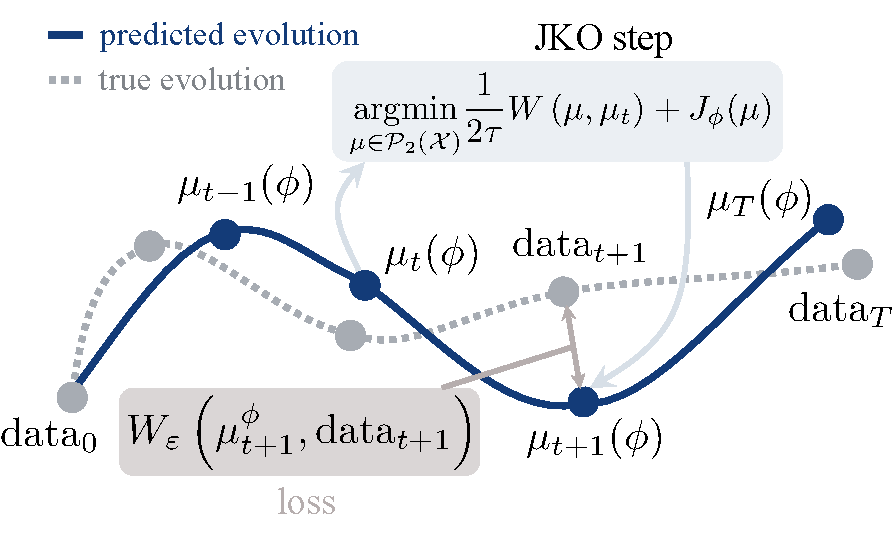
\includegraphics[width=0.6\textwidth]{figures/fig_overview_jkonet.pdf}
    \caption{Given an observed trajectory $(\mathrm{data}_0,\dots,\mathrm{data}_T)$ of point clouds (gray), we seek parameters $\phi$ for the energy $J_\phi$ such that the predictions $\mu_1, \dots, \mu_T$ (blue) following a \acrshort{JKO} flow from $\mu_0=\mu_0$ are close the observed trajectory (gray), by minimizing (as a function of $\phi$) the sum of Wasserstein distances between $\mu_{t+1}$, the \acrshort{JKO} step from $\mu_{t-1}$ using $J_\phi$, and data $\mu_{t+1}$.}
    \label{fig:overview_jkonet}
\end{figure}


\section{\textsc{JKOnet}: A Proximal Optimal Transport Model} 

Given $T$ discrete measures $\mathrm{data}_0, \dots, \mathrm{data}_T$ describing the time evolution of a population, we posit that such an evolution follows a \acrshort{JKO} flow for the free energy functional $J$, and assume that energy does not change throughout the dynamic. We parameterize the energy $J$ as a neural network with parameters $\phi$ and fit $\phi$ so that the \acrshort{JKO} flow model matches the observed data. 

Fitting parameter $\phi$ with a reconstruction loss requires, using the chain rule, being able to differentiate the \acrshort{JKO} step's output w.r.t. $\phi$ (see \cref{fig:overview_jkonet}), and more precisely provide a way to apply that transpose Jacobian to an arbitrary vector when using reverse-mode differentiation. To achieve this, we introduce a novel approach to numerically solve \acrshort{JKO} flows using \acrshortpl{ICNN} (\cref{sec:jko_icnn}), resulting in a bilevel optimization problem targeting the energy $J_\phi$ (\cref{sec:learn_energy}).

\subsection{Reformulation of JKO Flows via ICNNs} \label{sec:jko_icnn}
Given a starting condition $\mu_t$ and energy functional $J_\phi$, the \acrshort{JKO} step consists in producing a new measure $\mu_{t+1}$ implicitly defined as the minimizer of~\eqref{eq:jko}. Solving directly~\eqref{eq:jko} on the space of measures involves substantial computational costs. Different numerical schemes have been developed, e.g., based notably on Eulerian discretization of measures \citep{carrillo2021primal, benamou2016discretization}, and/or entropy-regularized optimal transport \citep{peyre2015entropic}. However, these methods are limited to small dimensions since the cost of discretizing such spaces grows exponentially. Except for the Eulerian approach proposed in \citep{peyre2015entropic}, obtained as the fixed point of a Sinkhorn-type iteration, the differentiation would also prove extremely challenging as a function of the energy parameter $\phi$.

\looseness=-1 To reach scalability and differentiability, we build upon the approach outlined in \citet{benamou2016discretization} to reformulate the \acrshort{JKO} scheme as a problem solved over convex functions, rather than on measures $\mu$. Effectively, this is equivalent to making a change of variables in~\eqref{eq:jko}: Introduce a (variable) convex function $\varphi$, and replace the variable $\mu$ by the variable $\nabla \varphi_{\sharp}\mu_t$. Writing
\begin{equation}\label{eq:en}
\begin{split}
\mathcal{E}_J(\mu, \nu) := J(\mu) +\frac{1}{2 \tau}W_2^2(\mu, \nu),\\
\end{split}
\end{equation}
this identity states that, assuming $\mu$ and $\nu$ being absolutely continuous w.r.t. Lebesgue measure that
$$\min_{\mu}\mathcal{E}_J(\mu,\nu) = \min_{\varphi \text{ convex}} \mathcal{F}_J(\varphi, \nu):= \mathcal{E}_J(\nabla \varphi_{\sharp}\nu, \nu)\,,$$
simplifying the Wasserstein term in \eqref{eq:en}, using the assumption that $\varphi$ is convex and the \nameref{thm:brenier}:
\begin{equation}\mathcal{F}_J(\varphi, \nu) = J(\nabla \varphi_{\sharp}\nu) +\frac{1}{2 \tau} \!\! \int\!\! \| x - \nabla \varphi(x) \|^2 d \nu(x)\label{eq:jko_psi}
\end{equation}

\begin{algorithm}[t]
\caption{\textsc{JKOnet}}
\label{algo:jkonet}
\begin{algorithmic}

   \STATE {\bfseries Input:} Dataset $\mathcal{D}=\{\{\mathrm{data}_t^0 \}_{t=0}^T, \ldots, \{\mathrm{data}_t^N \}_{t=0}^T\}$ of $N$ population trajectories, $\phi^0$ energy parameter initialization, $\theta^0$ ICNN parameter initialization, learning rates $\gamma_\theta$ and $\gamma_\phi$, step $\tau$, regularizer $\varepsilon$, tolerance $\alpha$, {\texttt{TeacherForcing}} flag
   \STATE {\bfseries Output:} Free energy $J_{\phi}$ explaining underlying population dynamics of snapshot data
   \smallskip
   
   \STATE $\phi\leftarrow \phi^0$
   \FOR{$\{\mathrm{data}_t\}_{t=0}^T \in \mathcal{D}$} 
   \FOR{$t \gets 0$ \textbf{to} $T-1$}

   \STATE $\theta\leftarrow \theta^0$

   \IF{\texttt{TeacherForcing} \textbf{or} $t=0$}
    \STATE $\nu \leftarrow \mathrm{data}_t$
   \ELSE
   \STATE $\nu \leftarrow \mu_t(\phi)$
   \ENDIF
   \WHILE{$\frac{\sum_i \norm{\nabla_{\theta_i}\mathcal{F}_{J_\phi}(\theta)}_2}{\sum_i \text{count}(\theta_i)} \ge \alpha$}
    
   \STATE $\theta \leftarrow \theta - \gamma_\theta \times \nabla_\theta \mathcal{F}_{J_\phi,\nu}(\theta)$
   \ENDWHILE
   \STATE $\mu_{t+1}(\phi) \leftarrow \nabla \varphi_{\theta \sharp} \nu$

   \STATE $\phi \leftarrow \phi - \gamma_\phi \times \nabla_\phi W_\varepsilon(\mu_{t+1}(\phi), \mathrm{data}_{t+1})$
   \ENDFOR
   \ENDFOR
	
\end{algorithmic}
\end{algorithm}

We pick an ICNN architecture to optimize over a restricted family of convex functions, $\{\varphi_{\theta}\}$, and define, starting from $\mu_0(\phi):=\mathrm{data}_0$, the recursive sequence for $t\geq 0$,
\begin{equation} \label{eq:next_pop}
\mu_{t+1}(\phi) := \nabla \varphi_{\theta^\star\!(\phi, \mu_t(\phi))\, \sharp}\, \mu_{t}(\phi)\,,
\end{equation}
with $\theta^\star(\phi, \mu_t)$ defined implicitly using $\phi$ and any $\nu$ as 
\begin{align} \label{eq:thetastar}
    \theta^\star(\phi, \nu):=\arg \min_{\theta} \mathcal{F}_J(\varphi_{\theta},\nu)
\end{align}

\paragraph{Strong convexity of $\varphi_\theta$.} The strong convexity and smoothness of a potential $\varphi$ impacts the regularity of the corresponding OT map $\nabla\varphi$ ~\citep{caffarelli2000monotonicity,figalli2010optimal}, since one can show that for a $\ell$-strongly convex, $L$-smooth $\varphi$ one has~\citep{paty2020regularity} that
$$
\ell \|x - y\| \leq \|\nabla\varphi(x) -\nabla\varphi(y)\|  \leq L\|x - y\|.
$$
While it is more difficult to enforce the $L$-smoothness of a neural network, and more generally its Lipschitz constants \citep{scaman2018lipschitz} it is easy to enforce its strong convexity, by simply adding a term $\ell \|x\|^2/2$ to the corresponding potential, or a residual rescaled term $\ell x$ to the output $\nabla\varphi(x)$. This approach can be used to enforce that the push-forward of the gradient of an ICNN does not collapse to a single point, maintaining spatial diversity.

\subsection{Learning the Free Energy Functional}  \label{sec:learn_energy}
The energy function $J_\phi : \mathcal{P}(\mathbb{R}^d) \rightarrow \mathbb{R}$ can be any parameterized function taking a measure as input. 
Since our model assumes that the observed dynamic is parameterized entirely by that energy (and the initial observation $\mu_0$), the more complex this dynamic, the more complex one would expect the energy $J_\phi$ to be. We focus in this first attempt on linear functions in the space of measures, that is expectations over $\mu$ of a vector-input neural network $E_\phi$
\begin{equation} \label{eq:energy}
    J_\phi(\mu) := \int E_\phi(x) d\mu(x),
\end{equation}
where $E_\phi:\mathbb{R}^d \rightarrow \mathbb{R}$ is a \acrfull{MLP}.


Inferring nonlinear energies accounting for population growth and decline, as well as interactions between points, using the formalism of \citep{de2019stochastic}, transformers~\citep{vaswani2017attention} or set pooling methods \citep{edwards2016towards, zaheer2017deep}, is an exciting direction for future work.

To address slow convergence and instabilities for dynamics with many snapshots, we use teacher forcing \citep{williams1989learning} to learn $J_\phi$ through time. In those settings, during training, $J_\phi$ uses the ground truth as input instead of predictions from the previous time step. At test time, we do not use teacher forcing.

\subsection{Bilevel Formulation of \textsc{JKOnet}}
Learning the free energy functional $J_\phi$ while solving each \acrshort{JKO} step via an ICNN results in a challenging bilevel optimization problem.
At each time step, the predicted dynamics are compared to the ground truth trajectory $(\mathrm{data}_0, \mathrm{data}_1, \dots, \mathrm{data}_T)$ with the entropy-regularized OT loss (see \ref{eq:ot-reg}),
\begin{align} \label{eq:fittingloss}
\begin{split}
    \min_\phi & \sum_{t=0}^{T-1} W_\varepsilon(\mu_{t+1}(\phi), \mathrm{data}_{t+1}), \\
    \text{s.t. } & \mu_{0}(\phi) := \mathrm{data}_0, \\
      & \mu_{t+1}(\phi) := \nabla \varphi_{\theta^\star\, \sharp}\, \mu_{t}(\phi)\,, \\
      & \theta^\star:=\arg \min_{\theta} \mathcal{F}_{J_{\phi}}(\varphi_{\theta},\mu_t(\phi))
\end{split}
\end{align}
The dependence of the Sinkhorn divergence losses in \eqref{eq:fittingloss} on $\phi$ only appears in the fact that the predictions $\mu_{t+1}(\phi)$ are themselves implicitly defined as solving a \acrshort{JKO} step parameterized with the energy $J_\phi$. 

\begin{figure}[t]
    \centering
    %\vskip-0.1cm
    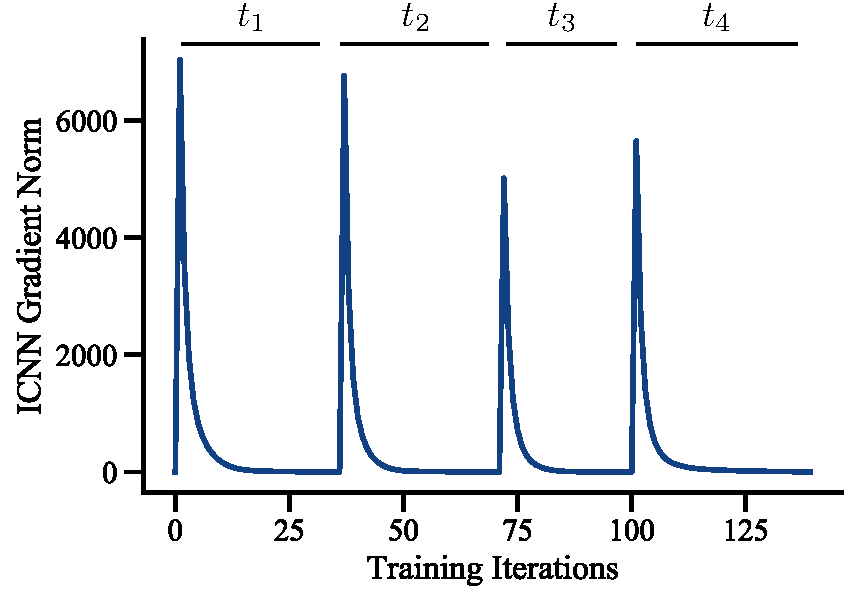
\includegraphics[width=.6\textwidth]{figures/fig_optimization_icnn.pdf}
    \caption{Optimization of the ICNN used in \acrshort{JKO} steps. The bumps correspond to a change in the outer iteration, and the smooth decrease in between corresponds to a single minimization~\eqref{eq:thetastar} of a time step $t_i$.}
    \label{fig:training_icnn}
\end{figure}

Learning  $J_\phi$ through the exclusive supervision of data observations requires therefore to differentiate the arg-minimum of a \acrshort{JKO} problem, down therefore through to the lower-level optimization of the ICNN. We achieve this by implementing a differentiable double loop in \texttt{JAX}, differentiating first the Sinkhorn divergence using the \texttt{OTT} package \citep{cuturi2022optimal}, and then backpropagating through the ICNN optimization by unrolling Adam steps \citep{kingma2014adam, metz2016unrolled, lorraine2020optimizing}.

\begin{figure*}[t]
\centering
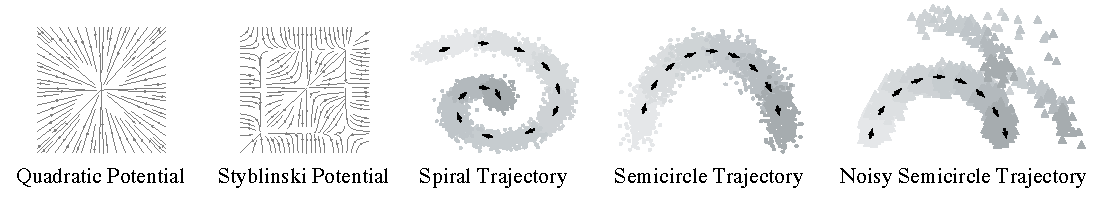
\includegraphics[width=1.0\textwidth]{figures/fig_task_overview_noise.pdf}
\caption{Overview on different tasks including trajectory- and potential-based dynamics.}
\label{fig:task_overview}
\end{figure*}

\paragraph{Inner loop termination.} A question that arises when defining $\mu_{t+1}(\phi)$ lies in the budget of gradient steps needed or allowed to optimize the parameters $\theta$ of the ICNN, before taking a new gradient step on $\phi$ in the outer loss. A straightforward approach in \texttt{JAX} \citep{jax2018github} would be to use a preset number of iterations with a \texttt{for} loop (\texttt{jax.lax.scan}). 
We do observe, however, that the number of iterations needed to converge in relevant scenarios can vary significantly with the ICNN architecture and/or the hardness of the underlying task.
We propose to use instead a differentiable fixed-point loop to solve each \acrshort{JKO} step up to a desired convergence threshold.
We measure convergence of the optimization of the ICNN via the average norm of the gradient of the \acrshort{JKO} objective w.r.t. the ICNN parameters $\theta$, i.e., $\sum_i \norm{\nabla_{\theta_i}\mathcal{F}_{J_\phi}(\theta_i, \phi)}_2/\sum_i \text{count}(\theta_i)$.
We observe that this approach is robust across datasets and architectures of the ICNN. An exemplary training curve for the \acrshortpl{ICNN} updated successively along a time sequence is shown in Figure~\ref{fig:training_icnn}.

\paragraph{Reverse-mode differentiation.} The Jacobian $\partial \mu_{t+1} / \partial\phi$ arising when computing the gradient $\nabla_\phi W_\varepsilon(\mu_{t+1}(\phi), \mathrm{data}_{t+1})$ is obtained by unrolling the while loop above. The gradient term of the Sinkhorn divergence w.r.t the first argument is given by the Danskin envelope theorem \citep{danskin2012theory}.

% The Jacobian $\partial \mu^\phi_{t+1} / \partial\phi$ that appears when computing $\nabla_\phi W_\varepsilon(\text{data}_{t+1}, \mu_{t+1}(\phi))$ is computed by unrolling the iterations of the while loop above.

\paragraph{Setting $\tau$ in \eqref{eq:jko_psi}.} 
In usual \acrshort{JKO} applications, $\tau$ needs to be tuned manually. Here, the energy $J_\phi$ is not fixed, but trained to fit data. Since we put no constraints on the scaling of $J_\phi$, $\tau$ can be set to $1$ without loss of generality, as the parameter $\phi$ will automatically adjust so that the scale of $J_\phi$ induces steps of a relevant length to fit data. This only holds (as with a usual \acrshort{JKO} step) if the trajectories are sampled regularly. For irregularly spaced time series, $\tau$ can be adapted at train and test time to the spacing of timestamps (shorter steps requiring larger $\tau$).


\begin{figure}[t]
     \centering
     \begin{subfigure}[t]{0.21\textwidth}
         \centering
         \caption{Quadratic \protect\newline potential.}
         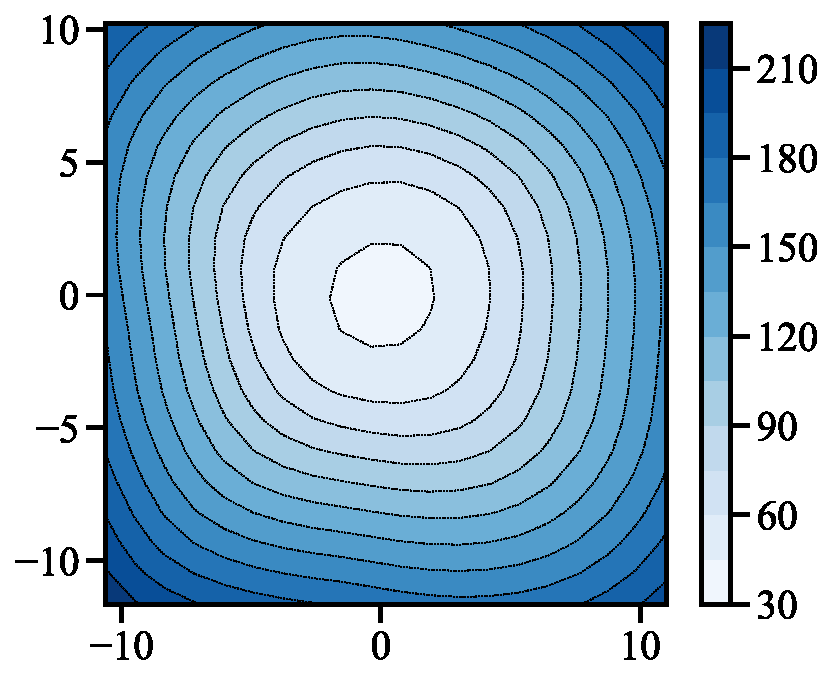
\includegraphics[width=\textwidth]{figures/fig_energy_implicit_quadratic.pdf}
     \end{subfigure}
     \hfill
     \begin{subfigure}[t]{0.21\textwidth}
         \centering
         \caption{Styblinski \protect\newline potential.}
         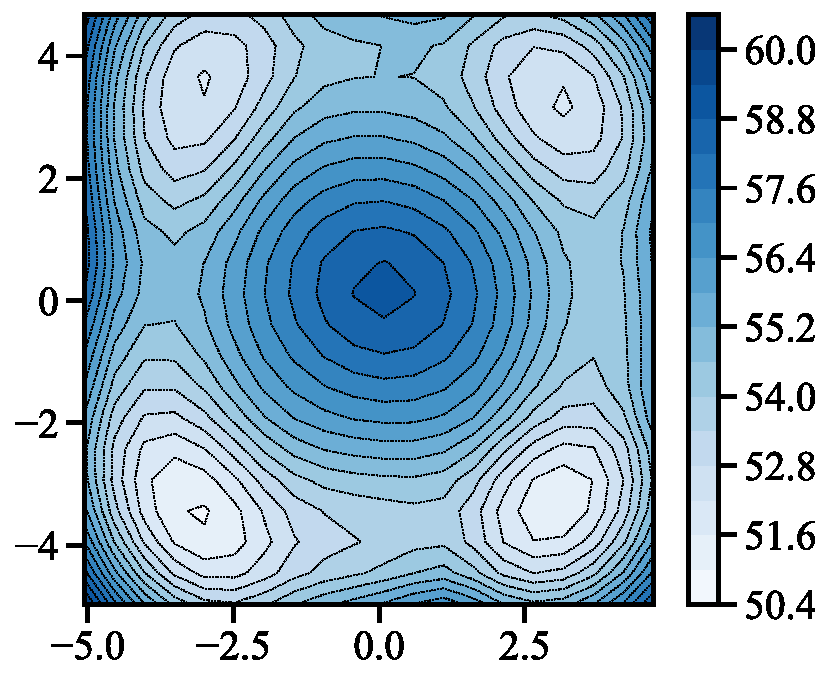
\includegraphics[width=\textwidth]{figures/fig_energy_implicit_styblinski.pdf}
     \end{subfigure}
     \hfill
     \begin{subfigure}[t]{0.22\textwidth}
         \centering
         \caption{Semicircle \protect\newline trajectory.}
         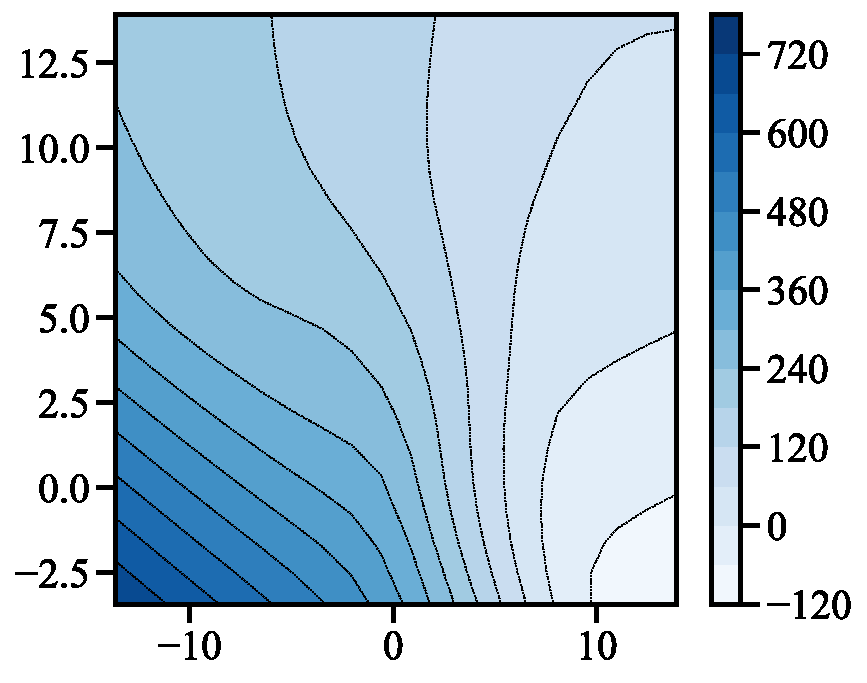
\includegraphics[width=\textwidth]{figures/fig_energy_implicit_semicircle_tf.pdf}
     \end{subfigure}
     \hfill
     \begin{subfigure}[t]{0.33\textwidth}
         \centering
         \caption{Predicted evolution \protect\newline on semicircle trajectory.}
         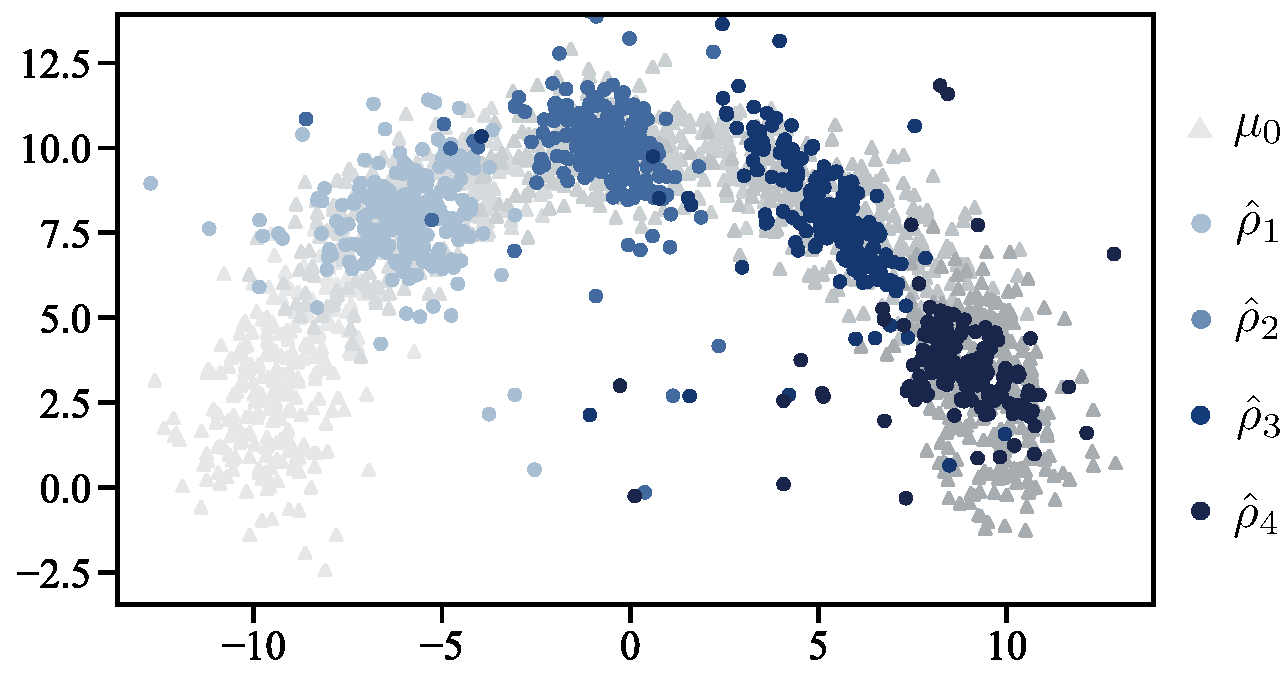
\includegraphics[width=\textwidth]{figures/fig_prediction_implicit_semicircle_tf.pdf}
     \end{subfigure}
	 \caption{\textbf{Results of \textsc{JKOnet} on potential- and trajectory-based dynamics.} (a)-(c) Contour plots of the energy functionals $J_\phi$ of \textsc{JKOnet} on potential- and trajectory-based population dynamics, color gradients depict the magnitude of $J_\phi$. (d) Predicted population snapshots ($\mu_1, \dots, \mu_4$) (blue) and data trajectory ($\mathrm{d}_0, \dots, \mathrm{d}_4)$ (gray).}
	 \label{fig:exp_jkonet_pot_traj}
\end{figure}
\begin{figure}[t]
     \centering
     \begin{subfigure}[t]{0.24\textwidth}
         \centering
         \caption{Forward method, \protect\newline teacher forcing.}
         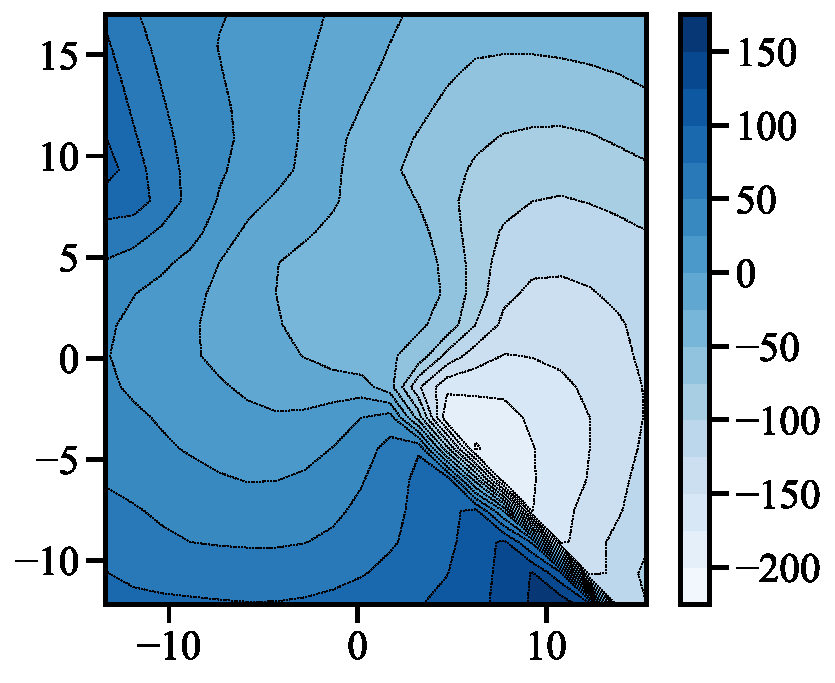
\includegraphics[width=\textwidth]{figures/fig_energy_explicit_spiral_tf.pdf}
     \end{subfigure}
     \hfill
     \begin{subfigure}[t]{0.24\textwidth}
         \centering
         \caption{Forward method, \protect\newline \emph{no} teacher forcing.}
         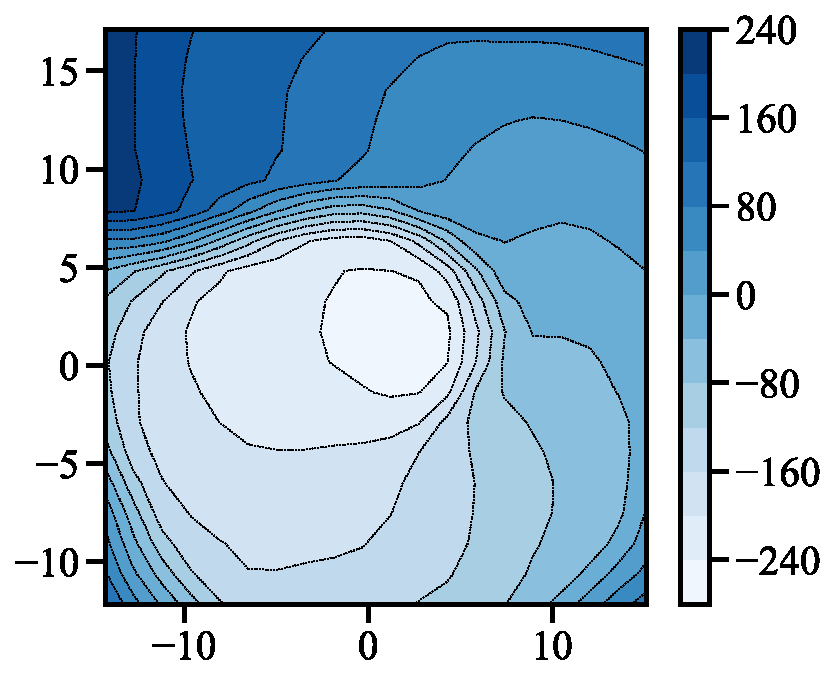
\includegraphics[width=\textwidth]{figures/fig_energy_explicit_spiral.pdf}
     \end{subfigure}
     \hfill
     \begin{subfigure}[t]{0.24\textwidth}
         \centering
         \caption{\textsc{JKOnet}, \protect\newline teacher forcing.}
         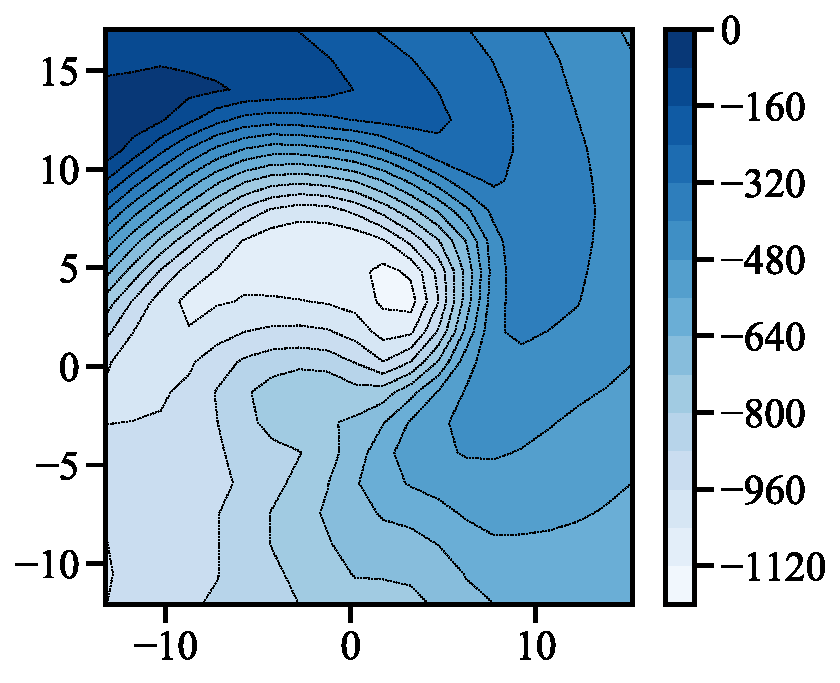
\includegraphics[width=\textwidth]{figures/fig_energy_implicit_spiral_tf.pdf}
     \end{subfigure}
     \hfill
     \begin{subfigure}[t]{0.24\textwidth}
         \centering
         \caption{\textsc{JKOnet}, \protect\newline \emph{no} teacher forcing.}
         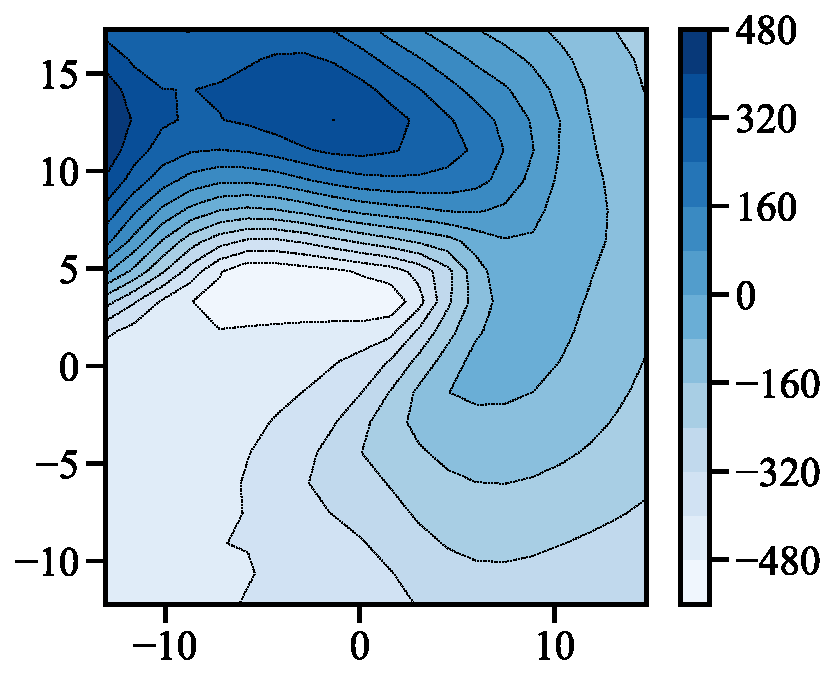
\includegraphics[width=\textwidth]{figures/fig_energy_implicit_spiral.pdf}
     \end{subfigure}
	 \caption{Comparison between energy functionals $J_\phi$ of the spiral trajectory task (see \ref{fig:task_overview}) between the forward method and \textsc{JKOnet}, trained with or without teacher forcing \cref{sec:learn_energy}). When using teacher forcing, the forward method overfits a gap in the lower-right corner of the spiral, outputting a highly irregular energy. When taking into account the entire trajectory recursively, the Forward method does better overall but is unable to recover an energy as precise as that returned by \textsc{JKOnet}.}
	 \label{fig:exp_comp_spiral}
\end{figure}

\begin{figure}[t]
     \centering
     \begin{subfigure}[t]{0.485\textwidth}
         \centering
         \caption{\textsc{JKOnet} (30\% corrupted data).}
         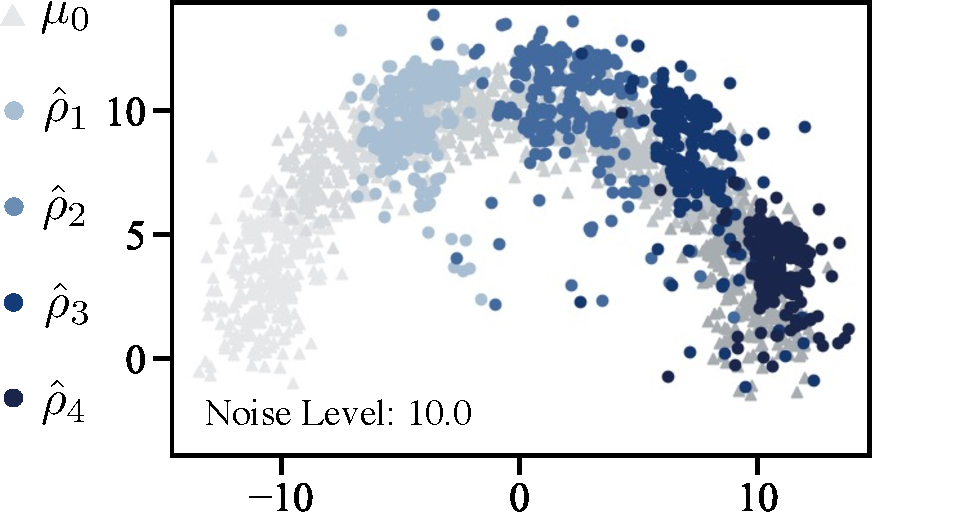
\includegraphics[width=\textwidth]{figures/fig_predictions_jko_noise.pdf}
     \end{subfigure}
     \hfill
     \begin{subfigure}[t]{0.46\textwidth}
         \centering
         \caption{Forward method (30\% corrupted data).}
         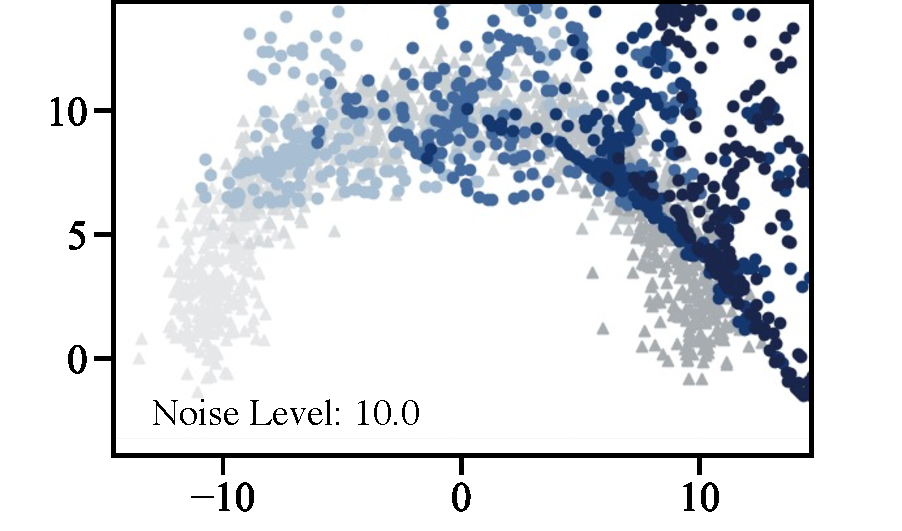
\includegraphics[width=\textwidth]{figures/fig_predictions_forward_noise.pdf}
     \end{subfigure}
     
     \begin{subfigure}[t]{0.485\textwidth}
         \centering
         \caption{$W_\varepsilon$ vs. noise level (20\% corrupted data).}
         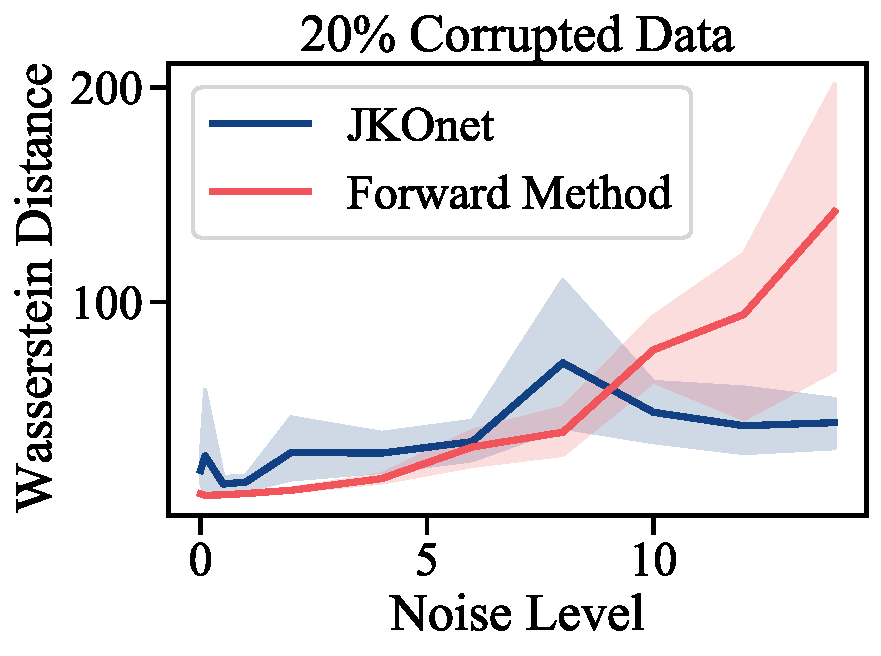
\includegraphics[width=\textwidth]{figures/fig_fb_comp_noise_20.pdf}
     \end{subfigure}
     \hfill
     \begin{subfigure}[t]{0.46\textwidth}
         \centering
         \caption{$W_\varepsilon$ vs. noise level (30\% corrupted data).}
         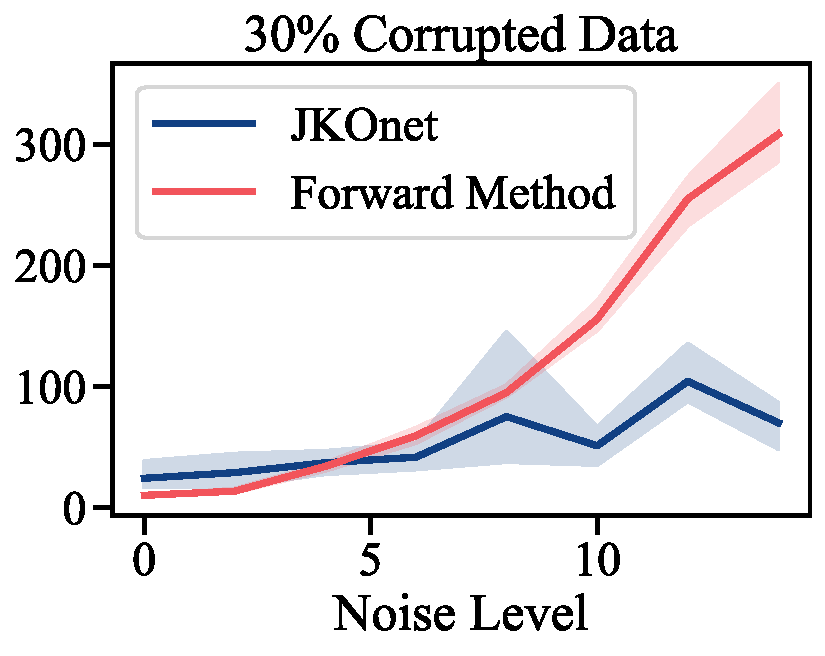
\includegraphics[width=\textwidth]{figures/fig_fb_comp_noise_30.pdf}
     \end{subfigure}
     \caption{Comparison between \textsc{JKOnet} and the forward method in settings of increasing noise on corrupted data on the semicircle trajectory task.}
     \label{fig:exp_comp_noise}
\end{figure}

\section{Empirical Evaluation} \label{sec:jkonet_evaluation}
In the following, we evaluate our method empirically on a variety of tasks. This includes recovering synthetic potential- and trajectory-based population dynamics (see \cref{fig:task_overview}), as well as the evolution of high-dimensional single-cell populations during a developmental process. 

\subsection{Synthetic Dynamics}
\label{sec:jkonet_synthetic}

\paragraph{Energy-driven trajectories.} The first task involves the evolution of partial differential equations with known potential. We hereby consider both convex (e.g., the quadratic function $J(x) = \|x\|^2_2$) and nonconvex potentials (e.g., Styblinski function) (see \cref{fig:task_overview}). These two-dimensional synthetic flows are generated using the Euler-Maruyama method~\citep{kloeden1992stochastic}. 
To recover the true potential via \textsc{JKOnet}, we parameterize both energy $J_\phi$ and ICNN $\varphi_\theta$ with linear layers ($\varepsilon = 1.0$, $\tau = 1.0$.
Figure~\ref{fig:exp_jkonet_pot_traj}a-b demonstrate \textsc{JKOnet}'s ability to recover convex and nonconvex potentials via energy $J_\phi$.

\paragraph{Arbitrary trajectories.}
As a sanity check, we evaluate if \textsc{JKOnet} can recover an energy functional $J_\phi$ from trajectories that are not necessarily arising from the gradient of an energy. Here, a 2-dimensional Gaussian moves along a predefined trajectory with nonconstant speed. 
We consider a line, a spiral, and movement along a semicircle (\cref{fig:task_overview}). As visible in Figure~\ref{fig:exp_jkonet_pot_traj}c (5 snapshots)], and Figure~\ref{fig:exp_comp_spiral}c-d (10 snapshots), \textsc{JKOnet} learns energy functionals $J_\phi$ that can then model the ground truth trajectories.
These trajectory-based dynamics are learned using the strong convexity regularizer ($\ell=0.8$, see \cref{sec:jko_icnn}).


\begin{table*}[t]
    \caption{Evaluation of predictive performance w.r.t. the entropy-regularized Wasserstein distance $W_\varepsilon$ \eqref{eq:ot-reg} of \textsc{JKOnet} and the forward method on the embryoid body scRNA-seq data per time step (using 3 runs).}
    \label{tab:exp_jkonet_cell_pred}
    \centering
\adjustbox{max width=.95\linewidth}{%
    \begin{tabular}{lcccc}
    \toprule
         \textbf{Method} & \multicolumn{4}{c}{\textbf{Prediction Loss ($W_\varepsilon$})} \\
         \cmidrule{2-5}
         & Day 6 to 9 & Day 12 to 15 & Day 18 to 21 & Day 24 to 27 \\
    \midrule
    \textbf{One Step Ahead} \\
        \tabindent Forward Method & $0.187 \pm 0.001$ & $0.162 \pm 0.010$ & $0.185 \pm 0.020$ & $0.203 \pm 0.004$ \\
        \tabindent \textsc{JKOnet} & $\mathbf{0.133 \pm 0.020}$ & $\mathbf{0.133 \pm 0.008}$ & $\mathbf{0.172 \pm 0.0130}$ & $\mathbf{0.169 \pm 0.004}$ \\
    \textbf{All Steps Ahead} \\
        \tabindent Forward Method & $0.225 \pm 0.023$ & $0.160 \pm 0.001$ & $0.171 \pm 0.016$ & $0.183 \pm 0.007$ \\
        \tabindent \textsc{JKOnet} & $\mathbf{0.148 \pm 0.015}$ & $\mathbf{0.144 \pm 0.013}$ & $\mathbf{0.154 \pm 0.024}$ & $\mathbf{0.138 \pm 0.034}$ \\
    \bottomrule
    \end{tabular}
}
\end{table*}

\paragraph{Comparison to forward methods.} \label{sec:eval_comp_fb}
Instead of parameterizing the next iteration $\mu_{t+1}(\phi)$ as we do in the \textsc{JKOnet} formulation~\eqref{eq:jko}, the \emph{forward} scheme states that the prediction at time $t+1$, $\eta_{t+1}$, can be obtained as $(\nabla F_\phi)_{\sharp} \eta_t(\phi)$, where $F_\phi$ is any arbitrary neural network, as considered in \citet{hashimoto2016learning}, namely $\eta_0:=\mu_0$ and subsequently $\eta_{t+1}(\phi):=(\nabla F_\phi)_{\sharp} \eta_t(\phi)$. Although OT still plays an important role in that paper, since the potential $F$ is estimated by minimizing a Sinkhorn loss $W_\varepsilon(\eta_{t+1},\mathrm{data}_{t+1})$, as we do in \eqref{eq:fittingloss}, the forward displacement operator $(\nabla F_\phi)_{\sharp}$ has no spatial regularity. Because of that, we observe that the forward method can get more easily trapped in local minima, and, in particular, overfits the training data as shown by a substantial decrease in performance in the presence of noise.
We demonstrate this by comparing the robustness of both \textsc{JKOnet} and the forward method to noise. For this, we corrupt $20\%$ or $30\%$ of the training data on the example of the semicircle trajectory with different levels of noise (see \cref{fig:task_overview}). We insist that noise is only added at training time, as random shifts on both feature dimensions, while we test on the original semicircle trajectory.
In low noise regimes, where train and test data are similar, the forward method overfits and performs marginally better than \textsc{JKOnet} (see \cref{fig:exp_comp_noise}c,d). As noise increases, the performance of the forward method deteriorates (\cref{fig:exp_comp_noise}b), while \textsc{JKOnet}, constrained to move points with OT maps, is robust (\cref{fig:exp_comp_noise}a).% This shows that the forward method is able to learn a network such that, on average, the ensemble of particles $(\nabla F_\phi)_{\sharp} \mu_t$ fits $\mu_{t+1}$, without, however

%In a second experiment, we evaluate the capacity of \textsc{JKOnet} and the forward method to extrapolate and generalize the learned trajectories, e.g., when vertically translating a line during test time (\cref{fig:task_overfitting}).
%Due to the less constrained energy, the \emph{forward} method perfectly resembles the seen trajectory during training but fails to extrapolate to shifted test data.

Second, we compare the resulting energy functionals $F_\phi$ and $J_\phi$ of the forward method and \textsc{JKOnet}, respectively, on the spiral trajectory (see \cref{fig:exp_comp_spiral}).
When learning long and complex population dynamics, teacher forcing improves training (see \cref{fig:exp_jkonet_pot_traj}c-d).
While facilitating the training of the forward method in some settings, it likewise results in wrong energy functionals $F_\phi$ (\cref{fig:exp_comp_spiral}a).
\textsc{JKOnet}, on the other hand, is able to globally learn the energy functional $J_\phi$, despite being only exposed to a one-step history of snapshots during training with teacher forcing (see \cref{fig:exp_comp_spiral}c).

\subsection{Single-Cell Dynamics}
\label{sec:jkonet_cell}

\begin{figure}[t]
     \centering
     \begin{subfigure}[t]{0.48\textwidth}
         \centering
         \caption{\acrshort{PCA} embedding of the embryoid body scRNA-seq data colored by the snapshot time.}
         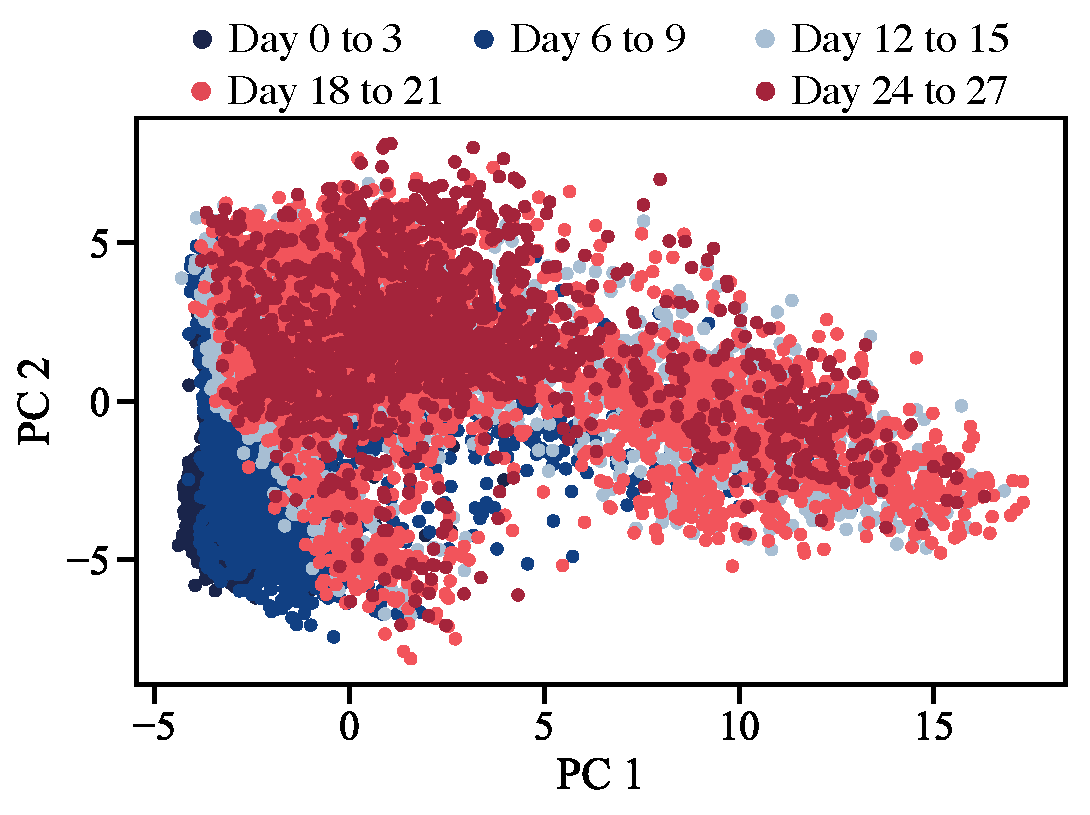
\includegraphics[width=\textwidth]{figures/fig_data_moon_days_full.pdf}
     \end{subfigure}
     \hfill
     \begin{subfigure}[t]{0.48\textwidth}
         \centering
         \caption{\acrshort{PCA} embedding of the embryoid body scRNA-seq data colored by the lineage branch class.}
         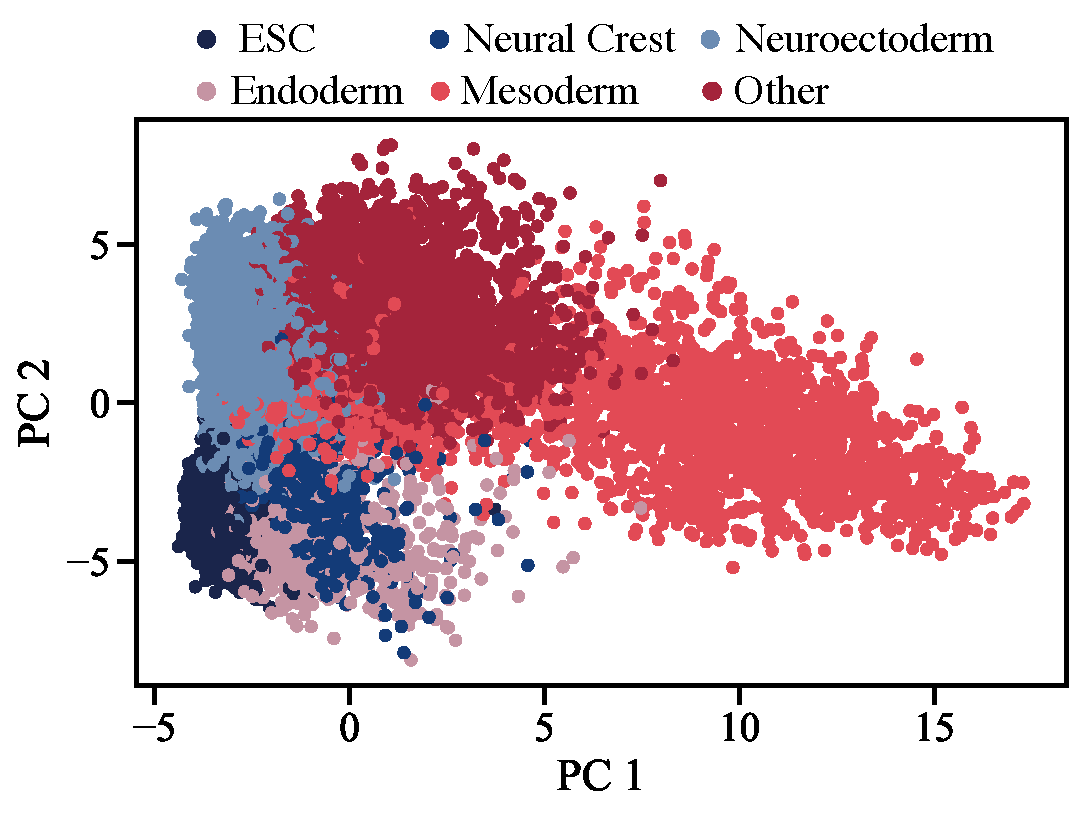
\includegraphics[width=\textwidth]{figures/fig_data_moon_Branches_full.pdf}
     \end{subfigure}

     \begin{subfigure}[t]{0.48\textwidth}
         \centering
         \caption{\acrshort{PCA} embedding of \textsc{JKOnet} predictions colored by the snapshot time.}
         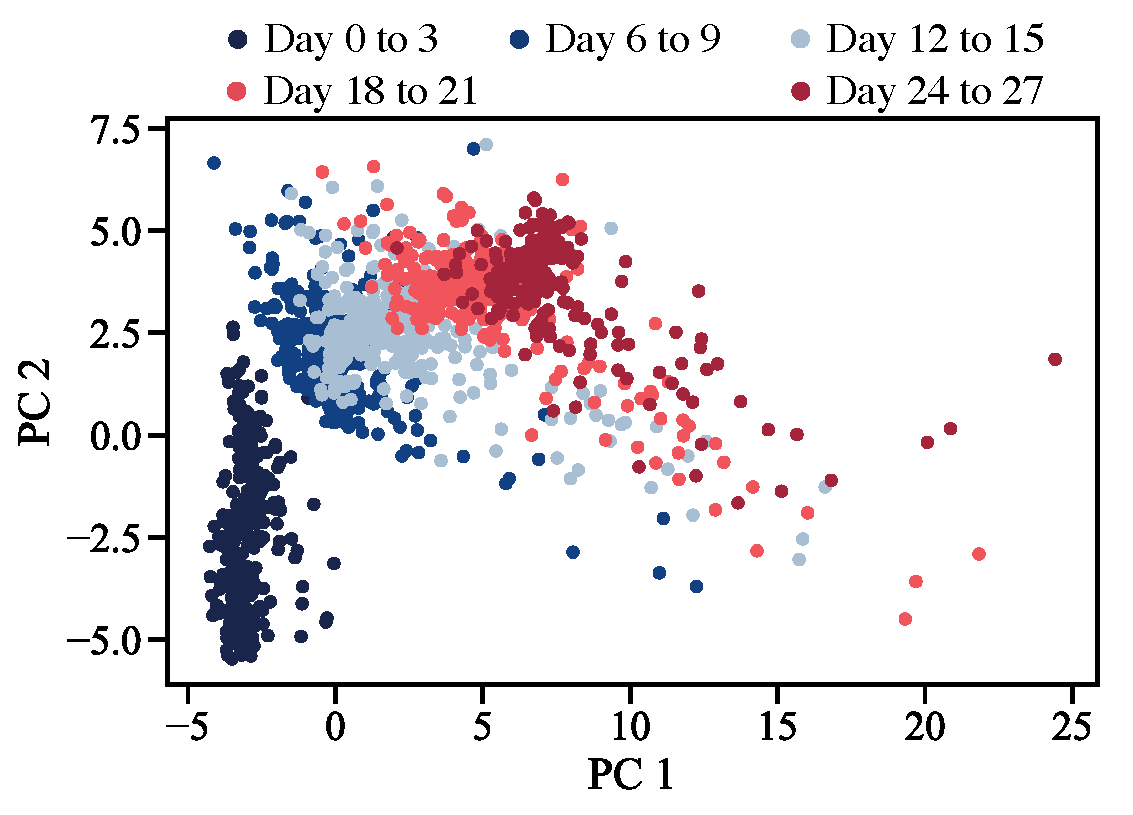
\includegraphics[width=\textwidth]{figures/fig_implicit_moon_pred_days.pdf}
     \end{subfigure}
     \hfill
     \begin{subfigure}[t]{0.48\textwidth}
         \centering
         \caption{\acrshort{PCA} embedding of \textsc{JKOnet} predictions colored by the lineage branch class.}
         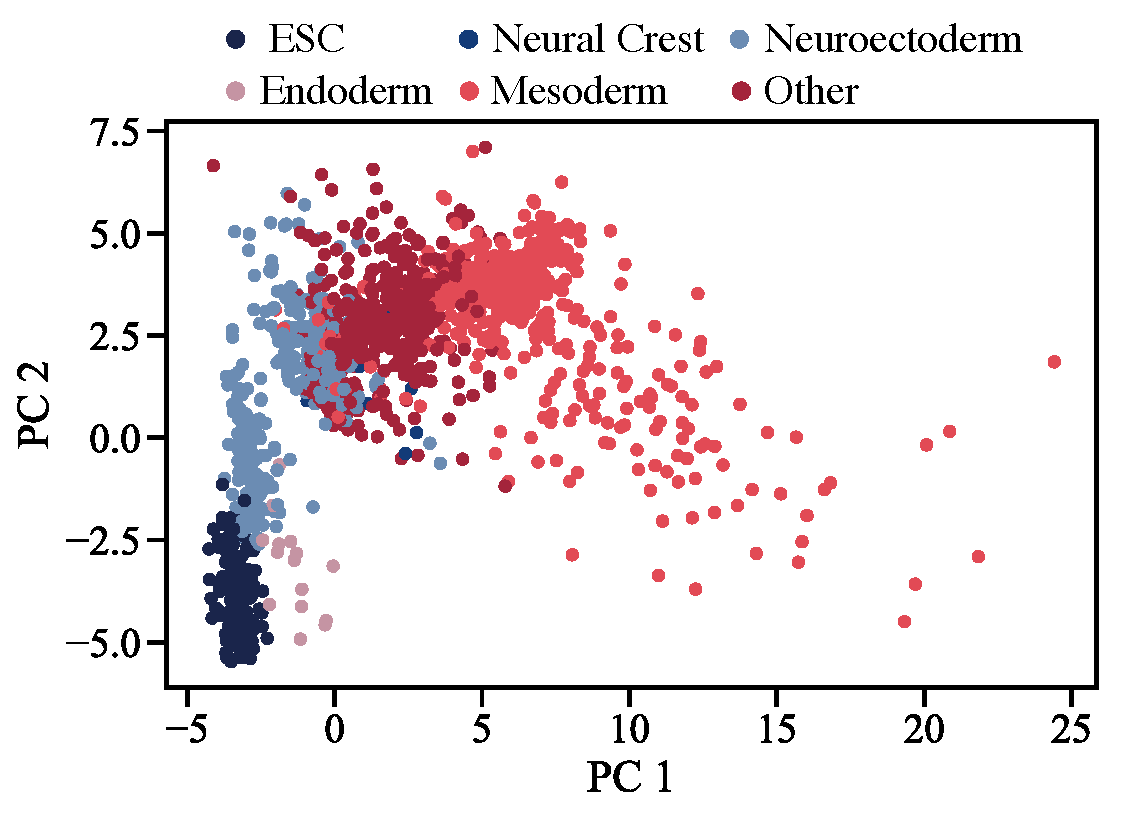
\includegraphics[width=\textwidth]{figures/fig_implicit_moon_pred_Branches.pdf}
     \end{subfigure}
	 \caption{Analysis of population dynamics predictions of \textsc{JKOnet} on the embryoid body scRNA-seq data.}
	 \label{fig:exp_jkonet_cell}
\end{figure}

\begin{figure}[t]
    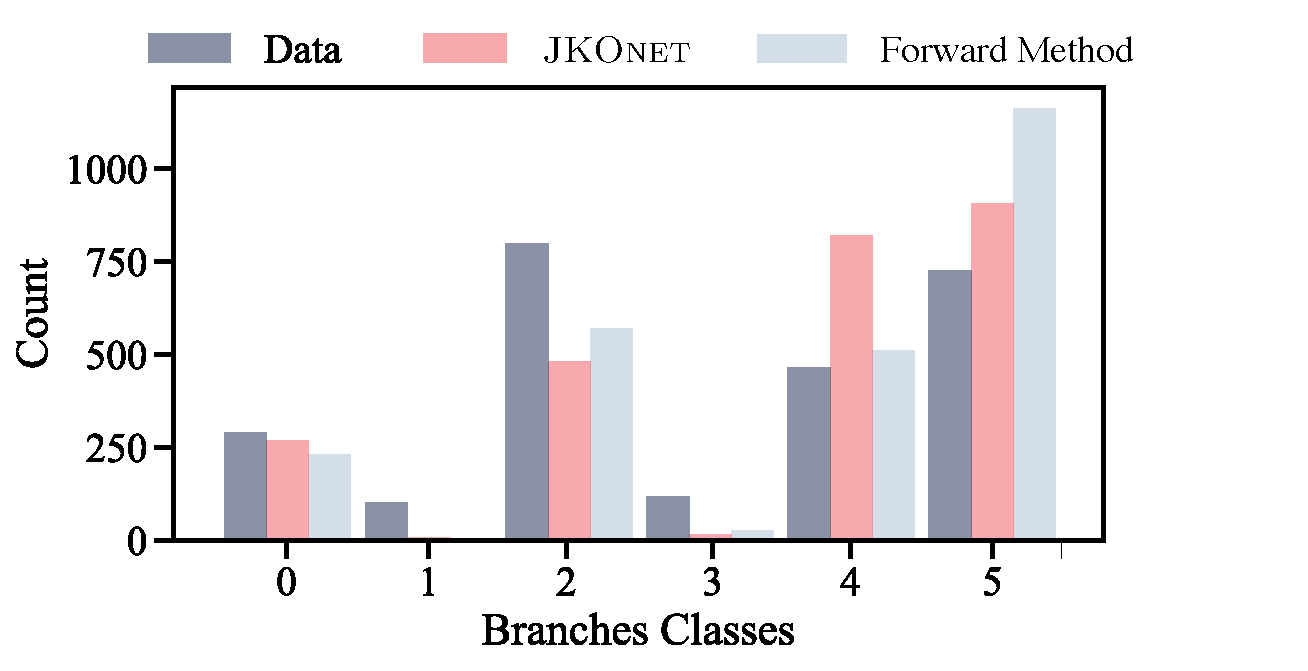
\includegraphics[width=.49\linewidth]{figures/fig_distribution_cell_types_Branches.pdf}
%    \captionof{figure}{Distribution of cell lineage branch classes in the data or  predicted by \textsc{JKOnet} or the forward method.}
	\quad
	\resizebox{.47\linewidth}{!}{%
    \begin{tabular}[b]{lcc}
    \toprule
         \textbf{Method} & \multicolumn{2}{c}{\textbf{Cell Lineage Classification}} \\
         & $\ell_1$ & $D_{\mathrm{H}}$ \\
    \midrule
    \textbf{One-Step Ahead} \\
        \tabindent Forward Method & $132.27 \pm 5.00$ & $0.026 \pm 0.002$ \\
        \tabindent \textsc{JKOnet} & $\mathbf{88.80 \pm 0.57}$ & $\mathbf{0.016 \pm 0.001}$ \\
    \textbf{All-Steps Ahead} \\
        \tabindent Forward Method & $\mathbf{185.47 \pm 12.18}$ & $0.033 \pm 0.002$ \\
        \tabindent \textsc{JKOnet} & $215.60 \pm 12.53$ & $0.034 \pm 0.004$ \\
    \bottomrule
    \end{tabular}
    }
\caption{Evaluation of cell lineage branch classification performance of \textsc{JKOnet} and the forward method on the embryoid body scRNA-seq data based on the $\ell_1$-distance of the histograms and the Hellinger distance $D_{\mathrm{H}}$ \eqref{eq:hellinger} of the predicted branch class distributions (using 3 runs).}
\label{tab:exp_jkonet_cell_class}
\end{figure}

We investigate the ability of \textsc{JKOnet} to predict the evolution of cellular and molecular processes through time.
% The advent of single-cell profiling technologies has enabled the generation of high-resolution single-cell data, making it possible to profile individual cells at different stages in their development. 
% A key difficulty in learning the evolution of cell populations is that a cell is (usually)  destroyed during a measurement. Thus, although one is able to collect features at the level of individual cells, the same cell cannot be measured twice. 
In the following, we are provided with a single-cell dataset of independent samples of distinct \emph{unaligned} distributions at each snapshot \textit{without} access to ground-truth single-cell trajectories. 
% The goal of learning individual dynamics is to identify ancestor and descendant cells and get a better understanding of biological differentiation or reprogramming mechanisms. 
More concretely, we apply \textsc{JKOnet} to embryoid body sc\acrshort{RNA-seq} data \citep{moon2019visualizing}, describing the differentiation of human embryonic stem cells grown as embryoid bodies into diverse cell lineages over a period of 27 days. During this time, cells are collected at 5 different snapshots (day 1 to 3, day 6 to 9, day 12 to 15, day 18 to 21, day 24 to 27) and measured via scRNA-seq (resulting in $15,150$ cells).
We run \textsc{JKOnet} as well as the baseline on the first 20 components of a \acrfull{PCA} of the $4,000$ highly differentiable genes. More details on the dataset are provided in \cref{app:dataset_moon}.
We split the dataset into train and test data ($\sim 15 \%$) and parameterize both energy $J_\phi$ and ICNN $\varphi_\theta$ with linear layers ($\varepsilon = 1.0$, $\tau = 1.0$).

\paragraph{Capturing spatio-temporal dynamics.}
Given the samples from the cell population at day 1 to 3 (i.e., $\mathrm{data}_0$), \textsc{JKOnet} learns the underlying spatiotemporal dynamics giving rise to the developmental evolution of embryonic stem cells. 
As no ground truth trajectories are available in the data, we use distributional distances, i.e., the entropy-regularized Wasserstein distance $W_\varepsilon$ \eqref{eq:ot-reg}, to measure the correctness of the predictions at each time step. 
We hereby measure the $W_\varepsilon$ discrepancy between data and predictions for one step ahead as well as inference of the entire evolution (all steps ahead) for each time step $t_i$, see results in Table~\ref{tab:exp_jkonet_cell_pred}. For details on the selected evaluation metrics, see \cref{app:evaluation_metrics}. \textsc{JKOnet} outperforms the forward method in terms of $W_\varepsilon$ \eqref{eq:ot-reg} distance for both one-step ahead and all-steps ahead predictions for all time steps. 
The performance of both methods is relatively stable even until days 24 to 27, i.e., the $W_\varepsilon$ distance does not significantly grow for future snapshots.
We further visualize the first two principal components of the entire dataset (\cref{fig:exp_jkonet_cell}a) and of \textsc{JKOnet}'s predictions on the test dataset ($\sim 500$ cells per snapshot, \cref{fig:exp_jkonet_cell}d). 

\paragraph{Capturing biological heterogeneity.}
Besides measuring the ability of \textsc{JKOnet} to model and predict the spatiotemporal dynamics of embryonic stem cells, we would like to guarantee, at a more macroscopic level, that \textsc{JKOnet} is also able to learn the cell's differentiation into various cell lineages.
Embryoid body differentiation covers key aspects of early embryogenesis and thus captures the development of \acrlongpl{ESC} into the mesoderm, endoderm, neuroectoderm, neural crest, and others.

Following \citet[Fig. 6, Suppl. Note 4]{moon2019visualizing}, we compute lineage branch classes (\cref{fig:exp_jkonet_cell}b) for all cells based on an initial $k$-means clustering ($k=30$) in a 10-dimensional embedding space using PHATE, a non-linear dimensionality reduction method capturing a denoised representation of both local and global structure of a dataset.
We then train a \acrfull{kNN} classifier ($k=5$) to infer the lineage branch class based on a 20-dimensional \acrshort{PCA} embedding of a cell (classes: ESC: 0, neural crest: 1, neuroectoderm: 2, endoderm: 3, mesoderm: 4, other: 5).

We analyze the captured lineage branch heterogeneity of the population predicted by \textsc{JKOnet} and the forward method by estimating the lineage branch class of each cell using the trained $k$-NN classifier. The predicted populations colored by the estimated lineage branch as well as the data with the true lineage branch labels are visualized in Figure~\ref{fig:exp_jkonet_cell}e and Figure~\ref{fig:exp_jkonet_cell}b, respectively.
The corresponding predicted and true distributions of lineage branch classes are shown in Figure~\ref{fig:exp_jkonet_cell}c.
To quantify how well \textsc{JKOnet} and the forward method capture  different cell lineage branches, we compute the $\ell_1$ distance between the  predicted and true histograms as well as the Hellinger distance 
\begin{equation} \label{eq:hellinger}
    D_{\mathrm{H}}(a, b) \defeq \frac{1}{2} \sum_{i=1}^{k}\left(\sqrt{a_{i}/\|a\|_1}-\sqrt{b_{i}/\|b\|_1}\right)^{2}
\end{equation}
between both true and predicted class discrete distributions $a$ and $b$.
Figure~\ref{fig:exp_jkonet_cell}c and Table~\ref{tab:exp_jkonet_cell_class} demonstrate that both, \textsc{JKOnet} and the forward method, capture most lineage branches during the differentiation of embryonic stem cells. Both methods, however, have difficulties recovering cells of the neural crest (class 1) and the endoderm (class 3), lineage branches that are scarcely represented in the original data. 
The analysis further suggests that both methods reduce in performance w.r.t. biological heterogeneity when predicting the entire trajectory (all steps ahead), instead of inferring the next snapshot only (one step ahead).


\section{Discussion}
We proposed \textsc{JKOnet}, a model to infer and predict the evolution of population dynamics using a proximal optimal transport scheme, the \acrshort{JKO} flow.
\textsc{JKOnet} solves local \acrshort{JKO} steps using \acrshortpl{ICNN} and learns the energy that parameterizes these steps by fitting \acrshort{JKO} flow predictions to observed trajectories using a fully differentiable bilevel optimization problem.
We validate its effectiveness through experiments on synthetic potential- and trajectory-based population dynamics and observe that it is far more robust to noise than a more direct Forward approach. We use \textsc{JKOnet} to infer the developmental trajectories of human embryonic stem cells captured via high-dimensional and time-resolved single-cell RNA-seq. 
Our analysis also shows that \textsc{JKOnet} captures diverse cell fates during the incremental differentiation of embryonic cells into multiple lineage branches.
Using proximal optimal transport to model real complex population dynamics thus makes for an exciting avenue of future work. Extensions could include modeling higher-order interactions among population particles in the energy function, e.g., cell-cell communication.
